\documentclass[12pt]{beamer}

\usepackage[T1]{fontenc}
\usepackage[francais]{babel}

\usepackage{lmodern}
\usepackage{fontspec}
\usepackage{graphicx}

\usepackage{hyperref}
\usepackage{minted}
\usepackage{tikz}

% BEGIN STYLE

\setbeameroption{hide notes}
\setbeamertemplate{note page}[plain]

\usetheme{default}
\beamertemplatenavigationsymbolsempty
\hypersetup{pdfpagemode=UseNone}

\setmonofont{Inconsolata}

\usepackage{epstopdf}

\usefonttheme{professionalfonts}
\usefonttheme{serif}
\usepackage{fontspec}
\setmainfont{Helvetica Neue}
\setbeamerfont{note page}{family*=pplx,size=\footnotesize}

\definecolor{latexblue}{RGB}{87,102,181}

\definecolor{background}{RGB}{39,8,11}
\definecolor{foreground}{RGB}{255,255,255}
\definecolor{title}{RGB}{255,255,255}
\definecolor{gray}{RGB}{159,255,197}
\definecolor{subtitle}{RGB}{159,255,197}
\definecolor{hilight}{RGB}{102,255,204}
\definecolor{vhilight}{RGB}{255,111,207}

\useinnertheme{rectangles}

\setbeamercolor{background canvas}{bg=background}
\setbeamercolor{titlelike}{fg=title}
\setbeamercolor{subtitle}{fg=subtitle}
\setbeamercolor{institute}{fg=gray}
\setbeamercolor{normal text}{fg=foreground,bg=background}
\setbeamercolor{item projected}{bg=foreground, fg=background}
\setbeamercolor{structure}{fg=foreground}
\setbeamercolor{subitem}{fg=foreground}
\setbeamercolor{itemize/enumerate subbody}{fg=foreground}

\setbeamertemplate{itemize subitem}{{\textendash}}

\setbeamerfont{itemize/enumerate subbody}{size=\footnotesize}
\setbeamerfont{itemize/enumerate subitem}{size=\footnotesize}

\setbeamertemplate{footline}{
  \raisebox{5pt}{\makebox[\paperwidth]{\hfill\makebox[20pt]{\color{gray}
\scriptsize\insertframenumber}}}\hspace*{5pt}}

\addtobeamertemplate{note page}{\setlength{\parskip}{12pt}}

\newminted{csharp}{bgcolor=background,fontsize=\footnotesize,mathescape}

\usemintedstyle{fruity}

% END STYLE

\title[Introduction au C\#]{\textbf{Introduction au C\#}}

\author{
  Quentin 'Neodyblue' Coelho\\
  Valentin 'toogy' Iovene\\
  Raphaël 'Shugo' Boissel
}

\date{28 novembre 2014}

\begin{document}

{
  \setbeamertemplate{footline}{} % no page number here
  \frame{
    \vspace{0.5cm}
    \begin{center}
      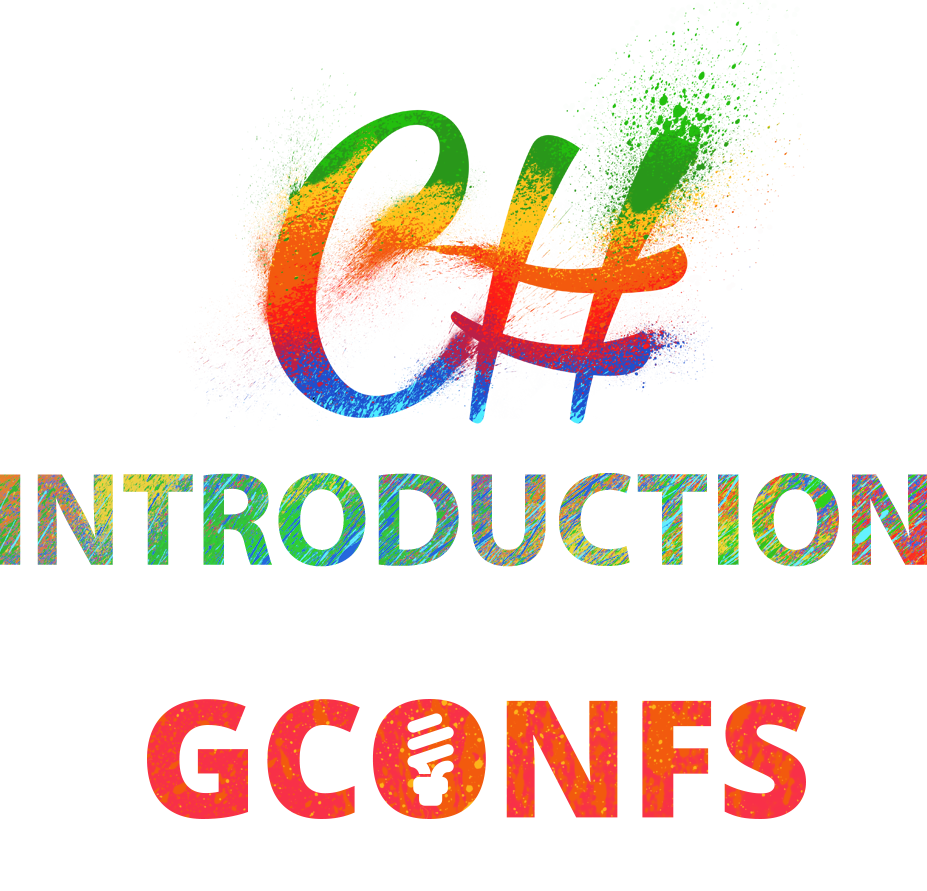
\includegraphics[scale=0.065]{img/cover.png}
    \end{center}
  }
}

\section*{Avant-propos}

\begin{frame}
    \frametitle{La conférence}
    \tableofcontents[pausesections]
\end{frame}


\section{Programmation Impérative}

\begingroup
\setbeamercolor{background canvas}{bg=title}
\begin{frame}
    \begin{center}
        \vspace{1cm}
        {\Large\color{background} Programmation \textbf{impérative}}
    \end{center}
\end{frame}
\endgroup



\section{Syntaxe C\#}

\begingroup
\setbeamercolor{background canvas}{bg=title}
\begin{frame}
    \begin{center}
        \vspace{1cm}
        {\Large\color{background}
            Syntaxe C\#
        }
    \end{center}
\end{frame}
\endgroup

\begin{frame}
  \begin{center}
    \vspace{1cm}
    Les variables
  \end{center}
\end{frame}

\setbeamercovered{transparent}
\begin{frame}[c]
  \frametitle{Déclaration}

  \begin{center}
    \begin{itemize}
      \item<+-> <type> <name>;
      \item<+-> <type> <name> = <valeur>;
      \item<+-> <type>[ ] <name>;
      \item<+-> <type>[ ] <name> = new <type>[<size>];
    \end{itemize}
  \end{center}
\end{frame}

\begin{frame}[fragile]
  \frametitle{Déclaration}

  \begin{center}{\large Exemples}\end{center}
  \begin{csharpcode*}{fontsize=\scriptsize}
    int i;
    string str;
    int a = 5;
    long verylong = 100000000000000;
    float val = 6.4f;
    double d = 4.2;
    string str2 = "Hello";
    int[] datas = new int[10];
  \end{csharpcode*}
\end{frame}

\begin{frame}[fragile]
  \frametitle{Manipulation}

  \begin{center}{\large Nombres}\end{center}
  \begin{csharpcode*}{fontsize=\scriptsize}
    int[] results = new int[2];
    int a = 4;
    bool vrai = true;
    bool faux = false;
    int b = 6;
    a = -1;
    results[0] = a + b; // [0] = 5
    b = 3;
    results[1] = a * b; // [1] = -3
  \end{csharpcode*}

  \pause

  \begin{center}{\large Strings}\end{center}
  \begin{csharpcode*}{fontsize=\scriptsize}
    string name = "Neodyblue";
    string text = "Welcome " + name + " !"; // "Welcome Neodyblue !"
  \end{csharpcode*}
\end{frame}

\begin{frame}
  \begin{center}
    \vspace{1cm}
    Les structures de contrôle
  \end{center}
\end{frame}

\begin{frame}[fragile]
  \frametitle{Les opérateurs de comparaison}

  \begin{itemize}
    \item<+-> == : 3 == 3
    \item<+-> != : 1 != 2
    \item<+-> < : 1 < 3
    \item<+-> > : 3 > 1
    \item<+-> <= : 1 <= 1
    \item<+-> >= : 4 >= 2
  \end{itemize}
\end{frame}

\begin{frame}[fragile]
  \frametitle{Le test}

  \begin{csharpcode*}{fontsize=\scriptsize}
    if (<booléen>)
    {
      // true
    }
    else
    {
      // false
    }
  \end{csharpcode*}
\end{frame}

\begin{frame}[fragile]
  \frametitle{Structures de contrôle}

  \begin{csharpcode*}{fontsize=\scriptsize}
    Console.WriteLine("Say my name !");
    string name = Console.ReadLine();

    if (name == "Heisenberg")
    {
      Console.WriteLine("You're goddamn right.");
    }
    else
    {
      Console.WriteLine("You lose !");
    }
  \end{csharpcode*}
\end{frame}

\begin{frame}
  \begin{center}
    \vspace{1cm}
    Les boucles
  \end{center}
\end{frame}

\begin{frame}[fragile]
  \frametitle{Le for}

  \begin{csharpcode*}{fontsize=\scriptsize}
    for (<init>; <booléen>; <step>)
    {
      // Do something
    }
  \end{csharpcode*}
\end{frame}

\begin{frame}[fragile]
  \frametitle{Les boucles}

  \begin{csharpcode*}{fontsize=\scriptsize}
    for (int i = 0; i < 10; ++i)
    {
      // This code will be executed 10 times
      // i values : 0, 1, 2, ..., 8, 9
    }
  \end{csharpcode*}
\end{frame}

\begin{frame}[fragile]
  \frametitle{Le while}

  \begin{csharpcode*}{fontsize=\scriptsize}
    while (<booléen>)
    {
      // Do something
    }
  \end{csharpcode*}
\end{frame}

\begin{frame}[fragile]
  \frametitle{Les boucles}

  \begin{csharpcode*}{fontsize=\scriptsize}
    string str = "";
    while (str.Length != 10)
    {
      str += "A";
    }
  \end{csharpcode*}
\end{frame}

\begin{frame}[fragile]
  \frametitle{Le do while}

  \begin{csharpcode*}{fontsize=\scriptsize}
    do
    {
      // Do something at least 1 time
    } while (<booléen>);
  \end{csharpcode*}
\end{frame}

\begin{frame}[fragile]
  \frametitle{Les boucles}

  \begin{csharpcode*}{fontsize=\scriptsize}
    string str = "";
    do
    {
      str = Console.ReadLine();
      // Do something with str
    } while (str != "exit");
  \end{csharpcode*}
\end{frame}

\begin{frame}
  \begin{center}
    \vspace{1cm}
    Les fonctions
  \end{center}
\end{frame}

\begin{frame}[fragile]
  \frametitle{Déclaration}

  \begin{csharpcode*}{fontsize=\scriptsize}
    <type> <name>(<parameter>)
    {
      // Code
    }
  \end{csharpcode*}
\end{frame}

\begin{frame}[fragile]
  \frametitle{Les fonctions}

  \begin{columns}[c]
    \column{2.2in}
    \begin{csharpcode*}{fontsize=\scriptsize}
      int sum(int a, int b)
      {
        return a + b;
      }
    \end{csharpcode*}

    \pause

    \begin{csharpcode*}{fontsize=\scriptsize}
      bool is_even(int n)
      {
        return n % 2 == 0;
      }
    \end{csharpcode*}

    \pause

    \column{2.3in}
    \begin{csharpcode*}{fontsize=\scriptsize}
      int div(int c, int d)
      {
        if (d == 0)
        {
          // FAIL
        }
        else
          return c / d;
      }
    \end{csharpcode*}
  \end{columns}
\end{frame}

\begin{frame}[fragile]
  \frametitle{Manipulation}

  \begin{csharpcode*}{fontsize=\scriptsize}
    int x = 5;
    int y = 11;

    int result_sum = sum(x, y); // result_sum = 16
    int result_div = div(x, y); // result_div = 0
    bool even = is_even(y); // even = false
  \end{csharpcode*}
\end{frame}

\begin{frame}[fragile]
  \frametitle{Les fonctions surchargées}

  \begin{csharpcode*}{fontsize=\scriptsize}
    void print(int n)
    {
      Console.WriteLine (n);
    }

    void print(int n, string msg)
    {
      Console.WriteLine (msg + " " + n);
    }
  \end{csharpcode*}
\end{frame}

\begin{frame}
  \begin{center}
    \vspace{1cm}
    Les collections
  \end{center}
\end{frame}

\begin{frame}[fragile]
  \frametitle{Les listes}

  \begin{csharpcode*}{fontsize=\scriptsize}
    List<<type>> <name> = new List<<type>>();
  \end{csharpcode*}
\end{frame}

\begin{frame}[fragile]
  \frametitle{Manipulation}

  \begin{csharpcode*}{fontsize=\scriptsize}
    List<string> words = new List<string>();
  \end{csharpcode*}

  \pause

  \begin{center}{\large Ajout et suppression}\end{center}
  \begin{csharpcode*}{fontsize=\scriptsize}
    words.Add("hello");
    words.Add("world");
    words.Add("test");
  \end{csharpcode*}
\end{frame}

\begin{frame}[fragile]
  \frametitle{Parcourir une collection}

  \begin{csharpcode*}{fontsize=\scriptsize}
    foreach (<type> <name> in <collection>)
    {
      // Do something with <name>
    }

    for (int i = 0; i < <collection>.Count; ++i)
    {
      // Do something with <name> and its index
    }
  \end{csharpcode*}
\end{frame}

\begin{frame}[fragile]
  \frametitle{Les collections}

  \begin{csharpcode*}{fontsize=\scriptsize}
    foreach (string current in words)
    {
      Console.WriteLine(current);
    }

    for (int i = 0; i < words.Count; ++i)
    {
      Console.WriteLine("[" + i + "]: " + words[i]);
    }
  \end{csharpcode*}
\end{frame}




\section{Programmation Orientée Objet \emph{(POO)}}

\begingroup
\setbeamercolor{background canvas}{bg=foreground}
\begin{frame}
    \begin{center}
        \vspace{1cm}
        {\Large\color{background}
        Programmation Orientée Objet \emph{(POO)}}
    \end{center}
\end{frame}
\endgroup

\begin{frame}[fragile]
  \begin{columns}[c]
    \column{2.3in}
    \begin{center}{\large Field (champ)}\end{center}
    \begin{csharpcode*}{fontsize=\scriptsize}
public class Circle
{
    public double radius;
    public string color;
}
    \end{csharpcode*}
    \pause
    \begin{center}{\large Method}\end{center}
    \begin{csharpcode*}{fontsize=\scriptsize}
public class Circle
{
    public double radius;
    public string color;

    public void setColor(string newColor)
    {
      this.color = newColor;
    }
}
    \end{csharpcode*}
    \column{2.2in}
    \pause
    \begin{center}
      {\large Property (propriété)}\\
      \emph{\scriptsize Snippet VS : propfull}
    \end{center}
    \begin{csharpcode*}{fontsize=\scriptsize}
public class Truc
{
    // backing field
    private int _attribut;

    public int Attribut // propriété
    {
        get { return _attribut; }
        set { _attribut = value; }
    }
}
    \end{csharpcode*}
  \end{columns}
\end{frame}

\begin{frame}[fragile]
    \begin{center}{\large Validation}\end{center}
    \begin{csharpcode*}{fontsize=\scriptsize}
class Thermostat
{
    private int _temperature; // backing field

    public int Temperature // propriété
    {
        get { return _temperature; }
        set
        {
            if (value >= 50)
                _temperature = 50;
            else
                _temperature = value;
        }
    }
}
    \end{csharpcode*}
\end{frame}

\begin{frame}[fragile]
    \begin{center}
        {\large Auto-propriété}\\
        \emph{\scriptsize Snippet VS : prop}
    \end{center}
    \begin{csharpcode}
public class Objet
{
    public int Attribut { get; set; };
}
    \end{csharpcode}
    \pause
    \begin{center}
        {\large Accès privé sur le \emph{set}}\\
        \emph{\scriptsize Snippet VS : propg}
    \end{center}
    \begin{csharpcode}
public class Objet
{
    public int Attribut { get; private set; };
}
    \end{csharpcode}
\end{frame}

\begin{frame}[fragile]
    \begin{center}{\large Interface}\end{center}
    \begin{csharpcode*}{fontsize=\scriptsize}
interface IBicycle
{
     string BrandName { get; set; }

     void Brake();
}
    \end{csharpcode*}
    \pause
    \begin{csharpcode*}{fontsize=\scriptsize}
class BlueBicycle : IBicycle
{
    private string _brandName;

    public string BrandName {
        get { return _brandName; }
        set { _brandName = lowerCase(value); }
    }

    void Brake() {
        // Braaaaaake! :o
    }
}
    \end{csharpcode*}
\end{frame}

\begingroup
\setbeamercolor{background canvas}{bg=foreground}
\begin{frame}
  \begin{center}
      \vspace{1.1cm}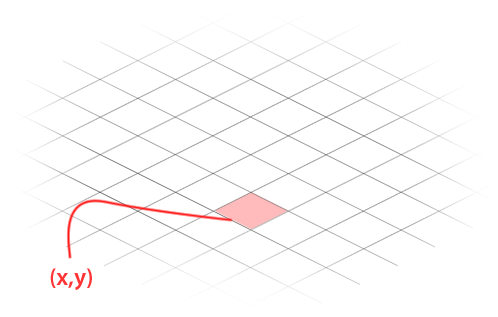
\includegraphics[scale=0.4]{img/map.png}
  \end{center}
\end{frame}

\begin{frame}
  \begin{center}
      \vspace{1.1cm}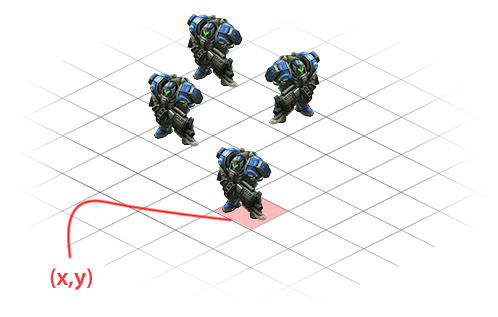
\includegraphics[scale=0.4]{img/unit.png}
  \end{center}
\end{frame}
\endgroup

\begin{frame}[fragile]
\begin{center}{\large Modélisation d'une unité}\end{center}
  \begin{csharpcode*}{fontsize=\scriptsize}
class Unit
{
    public Tuple<int,int> Position { get; set; }

    public int HealthPoints { get; set; }
    private int _maxHealthPoints;

    public int Speed { get; private set; }

    public int Dps { get; private set; }

    public void Move(Tuple<int,int> destination)
    {
        // Bouger
    }

    public void Die()
    {
        // Mourir
    }
}
  \end{csharpcode*}
\end{frame}

\begingroup
\setbeamercolor{background canvas}{bg=foreground}
\begin{frame}
  \begin{center}
    \vspace{1.4cm}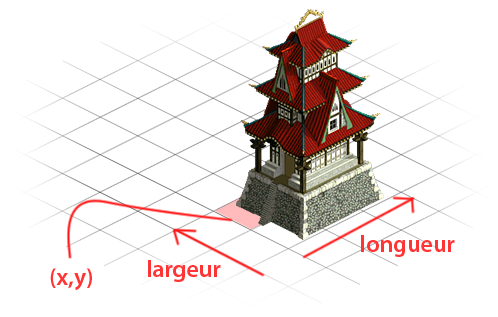
\includegraphics[scale=0.4]{img/building.png}
  \end{center}
\end{frame}
\endgroup


\begin{frame}[fragile]
\begin{center}{\large Modélisation d'un bâtiment}\end{center}
        \begin{csharpcode*}{fontsize=\scriptsize}
class Building
{
    public Tuple<int,int> Position { get; private set; }
    public Tuple<int,int> Size { get; private set; }

    public List<Unit> Units { get; set; }

    public int HealthPoints { get; set; }
    private int _maxHealthPoints;

    public void Die()
    {
        // Mourir
    }
}
        \end{csharpcode*}
\end{frame}

\begin{frame}[fragile]
  \begin{columns}[c]
    \column{2.3in}
    \begin{csharpcode*}{fontsize=\tiny}
class Unit
{
    public Tuple<int,int> Position { get; set; }

    public int HealthPoints { get; set; }
    private int _maxHealthPoints;

    public int Speed { get; private set; }

    public int Dps { get; private set; }

    public void Move(Tuple<int,int> destination)
    {
        // Bouger
    }

    public void Die()
    {
        // Mourir
    }
}
    \end{csharpcode*}
    \column{2.5in}
    \begin{csharpcode*}{fontsize=\tiny}
class Building
{
    public Tuple<int,int> Position { get; private set; }
    public Tuple<int,int> Size { get; private set; }

    public List<Unit> Units { get; set; }

    public int HealthPoints { get; set; }
    private int _maxHealthPoints;

    public void Die()
    {
        // Mourir
    }
}
    \end{csharpcode*}
  \end{columns}
\end{frame}

\begin{frame}[fragile]
    \begin{columns}[c]
        \column{2.3in}
        %\begin{center}{\large Classe Abstraite}\end{center}
        \begin{csharpcode*}{fontsize=\scriptsize}
abstract class GameItem
{
    public Tuple<int,int> Position
        { get; private set; }

    public int HealthPoints
        { get; set; }

    private int _maxHealthPoints;

    public abstract void Die();
}
        \end{csharpcode*}
        \pause
        \begin{csharpcode*}{fontsize=\scriptsize}
class Building : GameItem
{
    public Tuple<int,int> Size
        { get; private set; }

    public List<Unit> Units
        { get; set; }

    public override void Die()
    {
        // Mourir
    }
}
        \end{csharpcode*}
        \column{2.3in}
        \pause
        \begin{csharpcode*}{fontsize=\scriptsize}
class Unit : GameItem
{
    public int Speed
        { get; private set; }

    public int Dps
        { get; private set; }

    public void Move(
        Tuple<int,int> destination)
    {
        // Bouger
    }

    public override void Die()
    {
        // Mourir
    }
}
        \end{csharpcode*}
        \pause
        \begin{center}{\large Héritage}\end{center}
    \end{columns}
\end{frame}

\begin{frame}[fragile]
  \begin{csharpcode*}{fontsize=\scriptsize}
class MyClass
{
    public void MyFonction()
    {
        List<GameItem> gameItems = new List<GameItem>();

        gameItems.Add(new Unit());
        gameItems.Add(new Building());
    }
}
    \end{csharpcode*}
\end{frame}

\begin{frame}[fragile]
\begin{center}{\large Virtual methods}\end{center}
  \begin{csharpcode*}{fontsize=\scriptsize}
abstract class Unit
{
    public virtual void Die()
    {
        // A single death is a tragedy; a million deaths is a statistic.
    }
}
  \end{csharpcode*}
  \pause
  \begin{csharpcode*}{fontsize=\scriptsize}
class Bomber : Unit
{
    public override void Die()
    {
        // Kill everyone around before actually dying

        base.Fonction(parameter);
    }
}
    \end{csharpcode*}
\end{frame}


\section{Quelques conseils}

\begingroup
\begin{frame}
    \begin{center}
        \vspace{1cm}
        {\Large\color{foreground}
            Quelques conseils
        }
    \end{center}
\end{frame}
\endgroup


\begin{frame}[c]
  \begin{center}
    {\Large Des choses pas claires ?}
  \end{center}
\end{frame}

\end{document}
